\documentclass{simple}

\title[Cuvintele au putere]{Cuvintele au putere}
\institute{InfoEducație 2017 (Gălăciuc, Vrancea)}
\author[Răzvan Deaconescu]{Răzvan Deaconescu \\
razvan.deaconescu@cs.pub.ro}
\date{3 august 2017}

\begin{document}

\frame{\titlepage}

\begin{frame}{Să vedem și să ascultăm}
  \centering
  World of Warcraft: Wrath of the Lich King trailer: \url{https://www.youtube.com/watch?v=BCr7y4SLhck}
\end{frame}

\begin{frame}{Napoleon dixit}
  \centering
  \textit{A man does not have himself killed for a half-pence a day or for a petty distinction; you must speak to the soul in order to electrify him.}\\
  \vspace{3mm}
  \hfill \textit{Napoleon Bonaparte}
\end{frame}

\begin{frame}{Să vedem și să ascultăm}
  \centering
  V for Vendetta: The Revolutionary Speech: \url{https://www.youtube.com/watch?v=KKvvOFIHs4k}
\end{frame}

\begin{frame}{Esop dixit}
  \centering
  povestea cu limbile
\end{frame}

\begin{frame}{Cuvinte}
  \pause
  \centering
  gri vs. sur vs. cenușiu\\
  \pause
  \begin{figure}
    \centering
    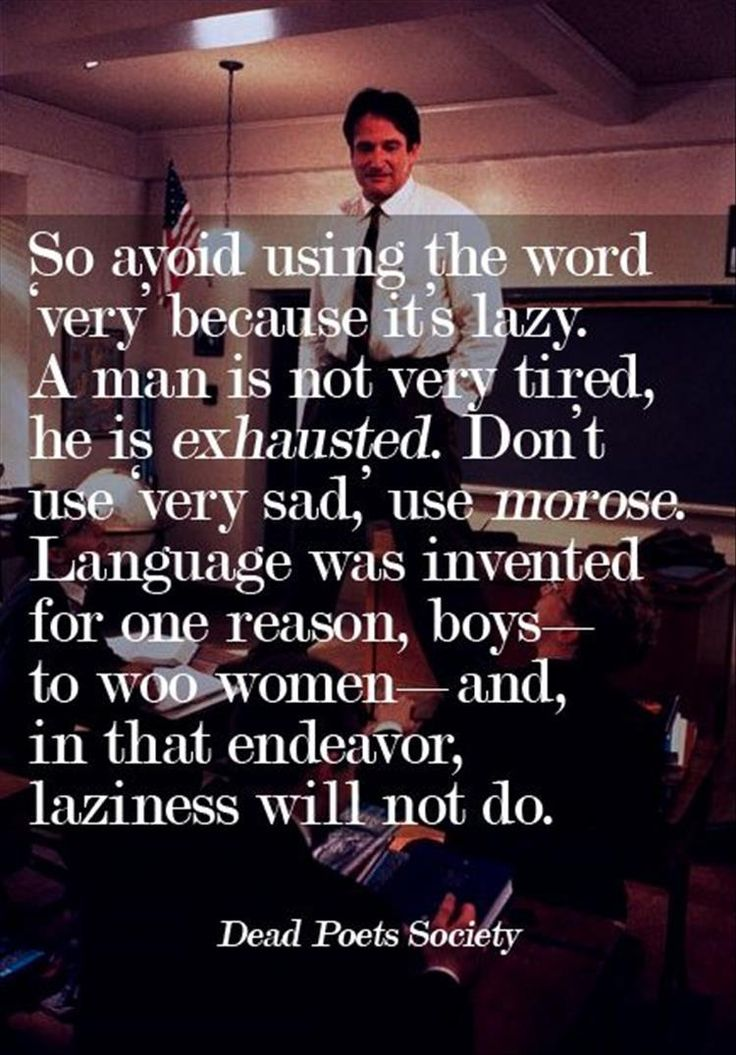
\includegraphics[width=0.4\textwidth]{img/dead-poets-society-lazy}
  \end{figure}
  \tiny
  \url{https://s-media-cache-ak0.pinimg.com/736x/6c/54/e6/6c54e6b4cd05585523d3ce5ae5a55574--robin-williams-writing-tips.jpg}
\end{frame}

\begin{frame}{Unde folosim cuvinte?}
  \centering
  \pause
  conversații, știri, anunțuri, articole, esee\\
  \pause
  \vspace{1cm}
  citate, slogan-uri, literatură, discursuri, dezbateri
\end{frame}

\begin{frame}{Cuvânt scris, cuvânt vorbit}
  \begin{itemize}
    \pause
    \item scriere vs. vorbire
    \pause
    \item mai multă putere are cuvântul vorbit
    \pause
    \item De ce există cuvânt scris?
    \pause
    \item citit ce a scris cineva, ascultat ce zice cineva, urmărit când și cum zice cineva
  \end{itemize}
\end{frame}

\begin{frame}{Tipuri de limbaj}
  \centering
  \pause
  verbal, para-verbal, non-verbal\\
  \pause
  \vspace{0.5cm}
  \textit{People discard what they hear in favor of what they see.}
\end{frame}

\begin{frame}{Ca să-l cităm pe Barack Obama}
  \pause
  \begin{center}
    \textit{You know I've got to talk about Donald Trump, right?}
  \end{center}
  \begin{itemize}
    \pause
    \item 8\% fapte, dar prinde
    \pause
    \item nepregătit, neinformat, fără viziune, fără o poziție politică consecventă, dar prinde
    \pause
    \item Cum?
      \begin{itemize}
        \pause
        \item cuvinte simple
        \pause
        \item agresivitate și dominanță
        \pause
        \item \textit{set the agenda}
        \pause
        \item lucrează pe psihic/emoție (Scott Adams: \textit{4D chess})
      \end{itemize}
  \end{itemize}
\end{frame}

\begin{frame}{Ce nu e bine aici?}
  \begin{figure}
    \centering
    
\includegraphics[width=0.4\textwidth]{img/love-trumps-hate}
  \end{figure}
  \begin{center}
    \tiny
    \url{http://www.imediaethics.org/wp-content/uploads/2015/12/lovetrumpshate.jpg}
  \end{center}
\end{frame}

\begin{frame}{Controlul conversației: rolul cuvintelor}
  \begin{center}
    \scriptsize
    suporter Hillary Clinton (\textit{0:13:08}):\\
    \url{https://www.youtube.com/watch?v=LibRNYJmZ-I&t=788s}\\
  \end{center}
  \pause
  \vspace{5mm}
  \begin{center}
    \textit{Fere libenter homines id quod volunt credunt.}\\
    \vspace{3mm}
    \hfill \textit{Gaius Julius Caesar}\\
    \vspace{5mm}
  \end{center}
  \begin{itemize}
    \pause
    \item argumentele factuale pot fi folosite doar în anumite situații și pentru un anumit tip de public/interlocutor
    \pause
    \item în mai multe situații merg exprimări de control psihologic/emoțional
  \end{itemize}
\end{frame}

\begin{frame}{Controlul conversației: Dincolo de cuvinte}
  \begin{itemize}
    \pause
    \item controlul liniștii
    \pause
    \item pauze
    \pause
    \item vorbit mai puțin
    \pause
    \item vorbit rar
    \pause
    \item vorbit mai tare
    \pause
    \item ruperi de ritm
    \pause
    \item calm
    \pause
    \item poziție relaxată
    \pause
    \item detașare
    \pause
    \item să pari în control, controlul emoțiilor
  \end{itemize}
\end{frame}

\begin{frame}{Ronald Reagan: The Great Communicator}
  \begin{center}
    \scriptsize
    Age Issue: \url{https://www.youtube.com/watch?v=LoPu1UIBkBc}\\
    \vspace{3mm}
    I Was a Democrat: \url{https://www.youtube.com/watch?v=yZMafGzDJdo}
  \end{center}
\end{frame}

\begin{frame}{Reframing}
  \begin{center}
    \scriptsize
    Tyrion Meets Shagga: \url{https://www.youtube.com/watch?v=BDwIDH9rFWo}\\
    \vspace{3mm}
    Robb Stark and Jaime Lannister: \url{https://www.youtube.com/watch?v=duWi6FR6PGw}
  \end{center}
\end{frame}

\begin{frame}{Ce s-a întâmplat aici?}
  \begin{center}
    \scriptsize
    Daenerys Meets with Tyrion and Jorah: \url{https://www.youtube.com/watch?v=zikSq-QiA7U}\\
    \vspace{1cm}
    \normalsize
    \pause
    flipping the script
  \end{center}
\end{frame}

\begin{frame}{Agree and Amplify}
  \centering
  \pause
  ești cam ipocrit\\
  \vspace{3mm}
  \pause
  ești cam scund\\
  \vspace{3mm}
  \pause
  ești cam copilăros\\
  \vspace{3mm}
  \pause
  vorbești cam repede\\
\end{frame}

\begin{frame}{Defectele ca armură}
  \centering
  \textit{Let me give you some advice bastard. Never forget what you are. The rest of the world will not. Wear it like armor, and it can never be used to hurt you.}\\
  \vspace{3mm}
  \hfill \textit{Tyrion Lannister (to Jon Snow)}
\end{frame}

\begin{frame}{Limbajul corpului / Body Language}
  \centering
  \pause
  limbajul non-verbal\\
  \vspace{3mm}
  \pause
  corelat cu mindset-ul (starea și percepția mentală)\\
  \vspace{3mm}
  \pause
  oamenii ,,te miros''
\end{frame}

\begin{frame}{Cum ajungi la public/interlocutor?}
  \begin{itemize}
    \pause
    \item creare (cuvinte) vs livrare (discurs)
    \pause
    \item grijă la public, mindset adecvat
  \end{itemize}
  \centering
  \pause
  \vspace{3mm}
  \textit{Un discurs este o discuție cu cineva, în care acel cineva este foarte important.}\\
  \vspace{3mm}
  \hfill \textit{Andrei Pleșu}\\
  \vspace{3mm}
  \begin{itemize}
    \pause
    \item keep it simple
    \pause
    \item autenticitate / convergență: fake it until you make it
    \pause
    \item percepție
    \pause
    \item emoție vs. informație: what Napoleon said, \textit{docere, movere, delectare}
    \pause
    \item ideile/informațiile concrete ne arată drumul, emoțiile ne împing înainte
  \end{itemize}
\end{frame}

\begin{frame}{Cum \textbf{nu} ajungi la public?}
  \centering
  \pause
  \textit{Sunt încântat de șansa de a conduce Microsoft România. Noul val de inovații din produsele, serviciile și soluțiile Microsoft și performanța echipei locale sunt ingredientele ce ne vor permite sa valorificăm oportunitățile extraordinare de creștere, cu același angajament pentru succesul clienților și partenerilor noștri.}\\
  \pause
  \begin{figure}
    
\includegraphics[width=0.6\textwidth]{img/promovare-spiru-haret}
  \end{figure}
\end{frame}

\begin{frame}{Spusul de povești / Storytelling}
  \centering
  \pause
  Ce urmărești în story telling?\\
  \pause
  \vspace{3mm}
  demo\\
  \pause
  \vspace{3mm}
  \textit{Mâna întinsă care nu spune o poveste, nu primește pomană.}\\
  \vspace{3mm}
  \hfill \textit{Pavel Puiuț (Filantropica, 2002)}
\end{frame}

\begin{frame}{Cuvinte, poezie, emoție}
  \begin{figure}
    \centering
    
\includegraphics[width=0.5\textwidth]{img/dead-poets-society-words-alive}
  \end{figure}
  \begin{center}
    \tiny
    \url{https://s-media-cache-ak0.pinimg.com/736x/a6/2d/85/a62d85757ae9854952281e9375314115--dead-poets-society-quotes-favorite-movie-quotes.jpg}
  \end{center}
\end{frame}

\begin{frame}{Vorbit bine}
  \pause
  mapă, logare, caracter, creere, sa creem, librărie, a compresa\\
  \vspace{5mm}
  \begin{itemize}
    \pause
    \item the right words (verbal)
    \pause
    \item the right tone (paraverbal)
    \pause
    \item the right posture (non-verbal)
    \pause
    \item the right frame: mindset, storytelling, convergență (non-verbal)
  \end{itemize}
\end{frame}

\begin{frame}{Cum ajungi la scris și vorbit bine}
  \centering
  \pause
  \textbf{citit, citit, citit}\\
  \vspace{3mm}
  \scriptsize
  \pause
  \textit{My mind is my weapon. My brother has his sword, King Robert has his warhammer and I have my mind\ldots{} and a mind needs books as a sword needs a whetstone if it is to keep its edge. That's why I read so much, Jon Snow.}\\
  \vspace{3mm}
  \hfill \textit{Tyrion Lannister (to Jon Snow)}
  \vspace{3mm}
  \begin{itemize}
    \pause
  \item experiență, vine cu vârsta, \textbf{poate fi accelerată}
    \pause
    \item urmărit filme: dialog și poveste (scenariu)
    \pause
    \item jocuri: dialog, poveste
    \pause
    \item urmărit stand-up-uri
    \pause
    \item \textbf{stat în lumina reflectoarelor}
    \pause
    \item dezbătut pe orice subiect
    \pause
    \item scris esee, blog-uri
    \pause
    \item citit și spus povești
    \pause
    \item observat ce faci tu și ajustat
  \end{itemize}
  \centering
  \vspace{3mm}
  \pause
  \textit{It usually takes me more than three weeks to prepare a good impromptu speech.}\\
  \vspace{3mm}
  \hfill \textit{Mark Twain}
\end{frame}

\begin{frame}{Făcut mișto-uri}
  \pause
  defecte ca armură\\
  \scriptsize
  \vspace{3mm}
  \pause
  \qquad Joffrey Baratheon: \textit{If I tell the Hound to cut you in half, he'll do it without a second thought.}\\
  \qquad Tyrion Lannister: \textit{That would make me the quarter-man. Just doesn't have the same ring to it.}\\
  \vspace{3mm}
  \normalsize
  \begin{itemize}
    \pause
    \item \textit{ball busting}
    \pause
    \item detașare, dispassionate, ZFG
    \pause
    \item să poți face mișto de orice credință (nu vei pierde controlul)
    \pause
    \item călire
  \end{itemize}
\end{frame}

\begin{frame}{Trolling}
  \centering
  \scriptsize
  \pause
  \url{http://www.urbandictionary.com/define.php?term=Trolling&defid=4250942}\\
  \vspace{5mm}
  \normalsize
  \pause
  De ce?
  \vspace{2mm}
  \begin{itemize}
    \pause
    \item estetica haosului
    \pause
    \item stârnirea de răspusuri emoționale
      \begin{itemize}
        \pause
        \item identificarea punctelor slabe (unde se ,,pișcă'' cineva)
        \pause
        \item stârnirea unor excese, argumente exagerate, demontarea argumentelor
        \pause
        \item controlul conversației
      \end{itemize}
  \end{itemize}
\end{frame}

\begin{frame}{De ce e important să știi despre cuvinte?}
  \begin{itemize}
    \pause
    \item cuvintele sunt parte din modul în care merge lumea
    \pause
    \item job-urile viitorului (multă automatizare)
    \pause
    \item persuasiune/negociere/manipulare
    \pause
    \item crearea și menținerea de relații
    \pause
    \item giving back/mentoring/passing knowledge
    \pause
    \item popularitate/apreciere/autoritate
    \pause
    \item înțelegerea mesajului și subtilităților, înțelegerea succesului
    \pause
    \item cuvintele sunt principalul mijloc de exprimare și transfer de emoție
  \end{itemize}
\end{frame}

\begin{frame}{Cuvintele au putere}
  \begin{figure}
    \centering
    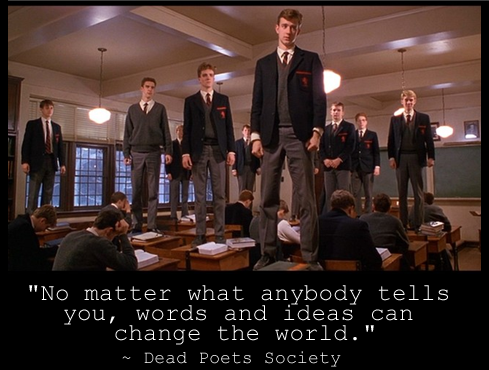
\includegraphics[width=0.7\textwidth]{img/dead-poets-society-words-change}
  \end{figure}
  \begin{center}
    \tiny
    \url{https://s-media-cache-ak0.pinimg.com/736x/43/ed/d5/43edd52f6d3b0c51925ff2fadd7e369e--peter-weir-peter-otoole.jpg}
  \end{center}
\end{frame}

\begin{frame}{Resurse și recomandări}
  \begin{itemize}
    \item slide-urile prezentării: \url{https://www.slideshare.net/razvandeaconescu/cuvintele-au-putere}
    \item Daniel Pink: A Whole New Mind: Why Right-Brainers Will Rule the Future
    \item Daniel Pink: To Sell Is Human: The Surprising Truth About Moving Others
    \item Robert Cialdini: Influence: The Psychology of Persuasion
    \item Joe Navarro: What Every Body Is Saying
    \item Baltasar Gracian y Morales: The Art of Worldly Wisdom
    \item Mike Cernovich: Gorilla Mindset
    \item film: Dead Poets Society (1989)
    \item Charisma on Command: \url{https://www.youtube.com/user/charismaoncommand}
  \end{itemize}
\end{frame}

\end{document}
